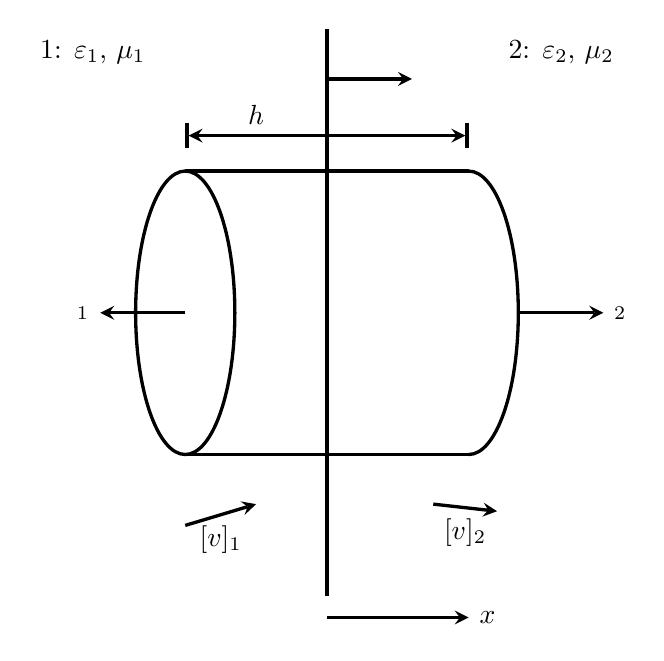
\begin{tikzpicture}[line width = 1.2pt, line join=round,x=1cm,y=1cm,>=stealth, scale = 0.9]
	% Medien und ihre Kennwerte
	\draw (-4.2,4) node [anchor=north west] {\circled{1}: $ \varepsilon_1 $, $ \mu_1$};
	\draw (4.2,4) node [anchor = north east] {\circled{2}: $ \varepsilon_2 $, $ \mu_2$};
	% linke Grundfläche
	\draw (-2,0) ellipse (0.7 and 2);
	% Beschriftung der Grundfläche
	\draw (-2,0.5) node [anchor=south] {$ \Flaeche{} $};
	\draw (-2,-0.5) node [anchor = north] {$ \volumen $};
	% rechte Grundfläche
	\draw (2.7,0) arc (0:90:0.7 and 2);
	\draw (2.7,0) arc (0:-90:0.7 and 2);
	% Mittelachse
	\draw (0,4) -- (0,-4);
	% obere und untere Begrenzung
	\draw (-2,2) -- (2,2);
	\draw (-2,-2) -- (2,-2);
	% Verschiebungsvektoren
	\draw[->] (-2,-3) -- (-1,-2.7) node [midway, below] {$ \DFeld[v]_1 $};
	\draw[->] (1.5,-2.7) -- (2.4,-2.8) node [midway, below] {$ \DFeld[v]_2 $};
	% x-Richtung
	\draw [->] (0,-4.3) -- (2,-4.3) node [anchor = west] {$ x $};
	% die Normalen
	\draw [->] (0,3.3) -- (1.2,3.3) node [anchor= west] {$ \normalenvektor $};
	\draw [->] (-2,0) -- (-3.2,0) node [anchor = east] {$ \normalenvektor_1 $};
	\draw [->] (2.7,0) -- (3.9,0) node [anchor = west] {$ \normalenvektor_2 $};
	% Höhe
	\draw [|<->|] (-2,2.5) -- (2,2.5) node [near start, above] {$ h $};
\end{tikzpicture}